% Figure 1: raw microdata, CP enrichment, and targeted MIP pool expansion.
\providecolor{ForestGreen}{rgb}{0.0,0.258,0.145}
\resizebox{0.98\textwidth}{!}{%
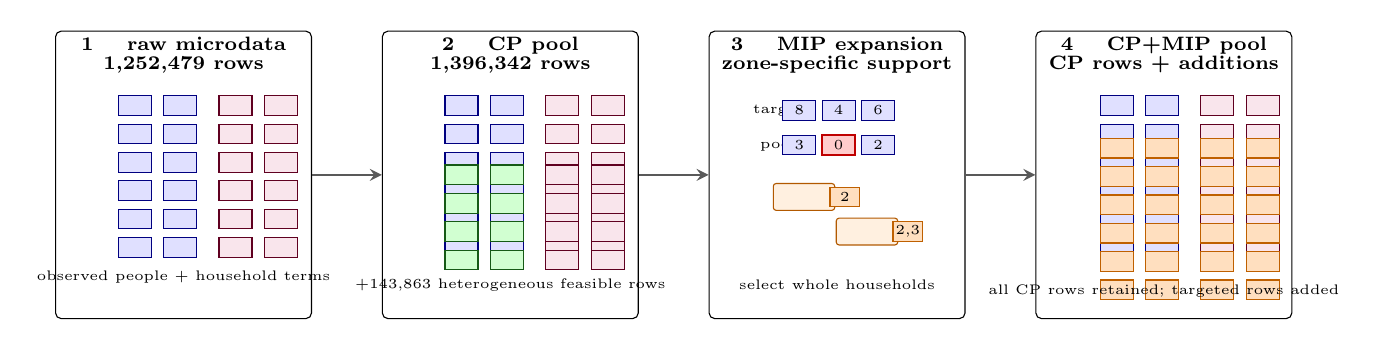
\begin{tikzpicture}[
  >=stealth,
  every node/.style={font=\small},
  panel/.style={draw, rounded corners=2pt, inner sep=5pt},
  title/.style={font=\scriptsize\bfseries, align=center},
  field/.style={draw, minimum width=0.42cm, minimum height=0.25cm,
                inner sep=0pt, align=center, font=\tiny},
  person/.style={field, fill=blue!12, draw=blue!50!black},
  household/.style={field, fill=purple!10, draw=purple!50!black},
  cpadd/.style={field, fill=green!18, draw=ForestGreen!65!black},
  mipadd/.style={field, fill=orange!25, draw=orange!75!black},
  zero/.style={field, fill=red!20, draw=red!75!black, line width=0.8pt},
  shell/.style={draw=black!65, rounded corners=1pt},
  arrow/.style={->, line width=0.9pt, draw=black!65}
]

% 1. Raw observed microdata.
\node[panel, minimum width=3.25cm, minimum height=3.65cm] (raw) at (0,0) {};
\node[title] at (0,1.52) {1 \quad raw microdata\\[-1pt]\scriptsize 1{,}252{,}479 rows};
\foreach \y in {0.88,0.52,0.16,-0.20,-0.56,-0.92} {
  \node[person] at (-0.62,\y) {};
  \node[person] at (-0.04,\y) {};
  \node[household] at (0.66,\y) {};
  \node[household] at (1.24,\y) {};
}
\node[font=\tiny] at (0,-1.30) {observed people + household terms};

% 2. CP construction adds broad feasible enrichment.
\node[panel, minimum width=3.25cm, minimum height=3.65cm] (cp) at (4.15,0) {};
\node[title] at (4.15,1.52) {2 \quad CP pool\\[-1pt]\scriptsize 1{,}396{,}342 rows};
\foreach \y in {0.88,0.52,0.16,-0.20,-0.56,-0.92} {
  \node[person] at (3.53,\y) {};
  \node[person] at (4.11,\y) {};
  \node[household] at (4.81,\y) {};
  \node[household] at (5.39,\y) {};
}
\foreach \y in {0.00,-0.36,-0.72,-1.08} {
  \node[cpadd] at (3.53,\y) {};
  \node[cpadd] at (4.11,\y) {};
  \node[household] at (4.81,\y) {};
  \node[household] at (5.39,\y) {};
}
\node[font=\tiny] at (4.15,-1.40) {+143{,}863 heterogeneous feasible rows};

% 3. MIP identifies a zone-specific support gap and candidate households.
\node[panel, minimum width=3.25cm, minimum height=3.65cm] (mip) at (8.30,0) {};
\node[title] at (8.30,1.52) {3 \quad MIP expansion\\[-1pt]\scriptsize zone-specific support};
\node[font=\tiny] at (7.55,0.82) {target};
\node[font=\tiny] at (7.55,0.38) {pool};
\foreach \x/\target/\cap in {7.82/8/3,8.32/4/0,8.82/6/2} {
  \node[person, minimum width=0.42cm] at (\x,0.82) {\target};
  \ifnum\cap=0
    \node[zero, minimum width=0.42cm] at (\x,0.38) {\cap};
  \else
    \node[person, minimum width=0.42cm] at (\x,0.38) {\cap};
  \fi
}
\node[shell, draw=orange!70!black, fill=orange!12,
      minimum width=0.78cm, minimum height=0.34cm, inner sep=0pt] at (7.88,-0.28) {};
\node[mipadd, minimum width=0.38cm] at (8.40,-0.28) {2};
\node[shell, draw=orange!70!black, fill=orange!12,
      minimum width=0.78cm, minimum height=0.34cm, inner sep=0pt] at (8.68,-0.72) {};
\node[mipadd, minimum width=0.38cm] at (9.20,-0.72) {2,3};
\node[font=\tiny] at (8.30,-1.40) {select whole households};

% 4. CP pool plus targeted MIP additions.
\node[panel, minimum width=3.25cm, minimum height=3.65cm] (expanded) at (12.45,0) {};
\node[title] at (12.45,1.52) {4 \quad CP+MIP pool\\[-1pt]\scriptsize CP rows + additions};
\foreach \y in {0.88,0.52,0.16,-0.20,-0.56,-0.92} {
  \node[person] at (11.85,\y) {};
  \node[person] at (12.43,\y) {};
  \node[household] at (13.13,\y) {};
  \node[household] at (13.71,\y) {};
}
\foreach \y in {0.34,-0.02,-0.38,-0.74,-1.10,-1.46} {
  \node[mipadd] at (11.85,\y) {};
  \node[mipadd] at (12.43,\y) {};
  \node[mipadd] at (13.13,\y) {};
  \node[mipadd] at (13.71,\y) {};
}
\node[font=\tiny] at (12.45,-1.48) {all CP rows retained; targeted rows added};

\draw[arrow] (raw.east) -- (cp.west);
\draw[arrow] (cp.east) -- (mip.west);
\draw[arrow] (mip.east) -- (expanded.west);

\end{tikzpicture}%
}
